\documentclass[twoside]{article}

\usepackage[english]{babel}
\usepackage{a4}
\usepackage{array}
\usepackage{amssymb}
\usepackage{amsmath}
\usepackage{graphicx}
\usepackage{fancyhdr}
\usepackage{array}
\usepackage{float}
\usepackage{hyperref}
\usepackage{xspace}
\usepackage{rotating}
\usepackage{dcolumn}
%\usepackage{portland}
\usepackage{color}
\usepackage{framed}

\setlength{\topmargin}{10mm}
\setlength{\topmargin}{-13mm}
% \setlength{\oddsidemargin}{0.5cm}
% \setlength{\evensidemargin}{0cm}
\setlength{\oddsidemargin}{1cm}
\setlength{\evensidemargin}{1cm}
\setlength{\textwidth}{14.5cm}
\setlength{\textheight}{23.8cm}

\pagestyle{fancyplain}
\addtolength{\headwidth}{0.6cm}
\fancyhead{}%
\fancyhead[RE,LO]{\bf MusrRoot --- open $\boldsymbol{\mu}$SR file format}%
\fancyhead[LE,RO]{\thepage}
\cfoot{--- Andreas Suter -- \today ---}
\rfoot{
\includegraphics[width=2cm]{PSI-Logo_narrow_blau}}

\DeclareMathAlphabet{\bi}{OML}{cmm}{b}{it}

\newcommand{\mean}[1]{\langle #1 \rangle}
\newcommand{\lem}{LE-$\mu$SR\xspace}
\newcommand{\musr}{$\mu$SR\xspace}
\newcommand{\trimsp}{\textsc{trim.sp}\xspace}
\newcommand{\mdu}{\texttt{MDU}\xspace}
\newcommand{\psibin}{\texttt{PSI-BIN}\xspace}
\newcommand{\musrroot}{\texttt{MusrRoot}\xspace}
\newcommand{\lemnpp}{\texttt{ROOT-NPP}\xspace}
\newcommand{\lemppc}{\texttt{ROOT-PPC}\xspace}
\newcommand{\rootcern}{\texttt{ROOT}\xspace}
\newcommand{\midas}{\texttt{Midas}\xspace}
\newcommand{\nexus}{\texttt{NeXus}\xspace}
\newcommand{\musrfit}{\texttt{musrfit}\xspace}
\newcommand{\anytwomany}{\texttt{any2many}\xspace}
\newcommand{\ie}{\emph{i.e.}\xspace}
\newcommand{\eg}{\emph{e.g.}\xspace}
\newcommand{\etc}{\emph{etc.}\xspace}
\newcommand{\redgreen}{\color{red}red\color{black}/\color{green}green\color{black}\xspace}
\newcommand{\tmrh}{\texttt{TMusrRunHeader}\xspace}
\newcommand{\tbrowser}{\texttt{TBrowser}\xspace}
\newcommand{\tfile}{\texttt{TFile}\xspace}
\newcommand{\tfolder}{\texttt{TFolder}\xspace}
\newcommand{\tobject}{\texttt{TObject}\xspace}
\newcommand{\tobjarray}{\texttt{TObjArray}\xspace}
\newcommand{\tobjstring}{\texttt{TObjString}\xspace}
\newcommand{\thonef}{\texttt{TH1F}\xspace}
\newcommand{\tstring}{\texttt{TString}\xspace}
\newcommand{\tstringvec}{\texttt{TStringVector}\xspace}
\newcommand{\tintvec}{\texttt{TIntVector}\xspace}
\newcommand{\tdoublevec}{\texttt{TDoubleVector}\xspace}
\newcommand{\tquant}{\texttt{TMusrRunPhysicalQuantity}\xspace}
\newcommand{\xml}{\texttt{XML}\xspace}

\newcolumntype{d}[1]{D{.}{.}{-1}}

\definecolor{shadecolor}{gray}{0.9}

\begin{document}
% Header info --------------------------------------------------
\thispagestyle{empty}
\noindent
\begin{tabular}{@{\hspace{-0.7cm}}l@{\hspace{6cm}}r}
\noindent
\includegraphics[width=3.4cm]{PSI-Logo_narrow_blau} &
  {\Huge\sf Memorandum}
\end{tabular}
%
\vskip 1cm
%
\begin{tabular}{@{\hspace{-0.5cm}}ll@{\hspace{4cm}}ll}
Datum:   & \today        &     & \\[3ex]
Von:     & Andreas Suter & An: & \\
Telefon: & +41\, (0)56\, 310\, 4238        &     & \\
Raum:    & WLGA / 119    & cc: & \\
e-mail:  & \verb?andreas.suter@psi.ch?, &&
\end{tabular}
%
\vskip 0.3cm
\noindent\hrulefill
\vskip 1cm
\begin{LARGE}
\noindent \textbf{MusrRoot File Format for $\boldsymbol{\mu}$SR}
\end{LARGE}
%
\tableofcontents
%

\section{Introduction}\label{sec:current}%

Until 2011 different \musr file formats were used within PSI. The bulk-\musr instruments were writing their data in the \psibin file format, which is a fixed binary format with rather stringent limitations. The \lem instrument was using a \rootcern based file format which was tightly tailored to the special needs of the \lem instrument. This situation was unsatisfactorily and hence it was decided to move forward to a open file format called \musrroot to be described in the following.

\section{Some basics concerning ROOT Files}\label{sec:basics-root-files}%

The \musr data acquisition systems at PSI are utilizing \midas \cite{Midas}. The \midas analyzer, which is responsible to build histograms, especially the \musr decay histograms, makes it very easy to build \rootcern \cite{ROOT} histogram objects (these are \thonef objects for \musr decay histograms). \rootcern is a \texttt{C++} object-oriented data mining frame work. These histograms can be collected and saved in \rootcern files (\tfile). In order to ease the understanding of the upcoming definitions, a few \rootcern related things shall be summaries here. For details concerning the \rootcern frame work documentation please check Refs.\cite{ROOT-Docu}.

\rootcern files (\tfile) are binary files which can hold any kind of objects. A \tfile is organized similarly to a directory structure of an operating system. Within the \rootcern framework, there is a \tfile browser available which allows to inspect these files. This browser (\tbrowser) will show all object saved in the \tfile directly, if they derive from \tobject.

The \musrroot file format to be described below is only using a small subset of possible \rootcern objects, namely:

\begin{itemize}
 \item \tfolder: This are the top level objects in the \musrroot file.
 \item \thonef: Hold the $\mu^\pm$-decay-histograms.
 \item \tobjarray: Holding collection of header information.
 \item \tobjstring: Holding the content of any header information.
\end{itemize}

\noindent Since all these objects are deriving form \tobject, they will be directly accessible via the \tbrowser. For instance, the $\mu^\pm$-decay-histograms can be directly plotted, are even fitted, out of the box.

\cleardoublepage

\section{\musrroot: an open $\boldsymbol{\mu}$SR file format}

As mentioned before, \rootcern files are open-file-format files meaning that they can contain more entries (and most probably will) than the ones specified in the following. The specified ones will be the mandatory ones for \emph{all} instruments. Before defining all mandatory entries, the \musrroot file structure shall be sketched.

\noindent The \musrroot file structure looks like:

\begin{verbatim}
histos ---|
          |- DecayAnaModule ---|
          |                    |- hDecay001
          |                    |- hDecay002
          |                    ...
          |
          |- SCAnaModule ---|
          ...               |- hSampleTemperature
                            |- hSampleMagneticField
                            ...
RunHeader ---|
             |- RunInfo
             |- DetectorInfo ---|
             |                  |- Detector001
             |                  |- Detector002
             |                  ...
             |
             |- SampleEnvironmentInfo
             |- MagneticFieldEnvironmentInfo
             |- BeamlineInfo
             ...
\end{verbatim}

\noindent where \texttt{hDecay001}, etc. are \rootcern histograms (to be more specific: \texttt{TH1F}), containing the \musr decay histograms. There can be as many as needed, especially there is no limitation about their length. The histogram object names will be \texttt{hDecayXXX}, where \texttt{XXX} (leading zero \texttt{int}, \ie \verb?%03d? in \texttt{C/C++} notation, starting with `1') is the histogram number. The title and name of the histogram (see description of the \texttt{TH1F} \rootcern class) contains the label of the histogram, like `top', `forward', etc. How many of these histograms are present is accessible through the \texttt{RunInfo} folder in which the necessary header information are found (details see next sections). The folder \texttt{SCAnaModule} contains histograms of some of the slow-control parameters, as for instance the sample temperature versus time, the applied field versus time, etc. Again the label of the histogram will give more specific information about its content.

\subsection{Run information contained in \texttt{RunHeader}}\label{sec:RunHeader}

The \texttt{RunHeader} contains all needed meta-information to describe a \musr-run. The list of the \emph{minimal number of required} ``folders'' of the \texttt{RunHeader} is given in the following structure:

\begin{small}
\begin{verbatim}
RunHeader (TFolder) ---|
                       |- RunInfo (TObjArray)
                       |- DetectorInfo (TObjArray)
                       |- SampleEnvironmentInfo (TObjArray)
                       |- MagneticFieldEnvironmentInfo (TObjArray)
                       |- BeamlineInfo (TObjArray)
\end{verbatim}
\end{small}

\noindent In brackets the object type is given. \texttt{RunInfo} contains most information relevant for the user and will be itemized Sec.\,\ref{sec:RunInfo} and \ref{sec:RunInfoRequired}. \texttt{DetectorInfo} contains detector specific information, like detector name, time zero bin, \etc (details in Sec.\,\ref{sec:DetectorInfoRequired}). \texttt{SampleEnvironmentInfo} (details in Sec.\,\ref{sec:SampleEnvironmentInfoRequired}), and \texttt{MagneticFieldEnvironmentInfo} (details in Sec.\,\ref{sec:MagneticFieldEnvironmentInfoRequired}) store additional, more detailed information concerning the sample environment. \texttt{BeamlineInfo} stores beamline relevant information (details in Sec.\,\ref{sec:BeamlineInfoRequired}).

Before elaborating more on the required items within this structure, a few words on the \rootcern types used here: \texttt{RunHeader} is a \tfolder object. All the ``sub-directory'' entries are of type \tobjarray and collect items of type \tobjstring or other \tobjarray (\ie sub-directories and sub-sub-directories, etc.).

\subsubsection{\texttt{RunInfo}}\label{sec:RunInfo}

\begin{small}
\begin{tabular}{l|l|l}
Name           & internal type & Comment \\ \hline\hline
Version        & \tstring      & GIT version of \tmrh \\
Generic Validator URL & \tstring & URL of the generic \musrroot validation xsd-file. \\
Specific Validator URL & \tstring & URL of the instrument specific validation xsd-file. \\
Generator      & \tstring      & Program which wrote the \musrroot file, \\
               &               & \eg \verb!nemu_analyzer! \\
Proposal Number & \verb!Int_t! & This item is optional, but if present, it \\
               &               & can only occur once. \\
Main Proposer  & \tstring      & This item is optional, but if present, \\
               &               & one or more main proposers are possible. \\
File Name      & \tstring      & File name of the \musrroot file, \\
               &               & \eg \verb!deltat_tdc_gps_4295.root! \\
Run Title      & \tstring      & \\
Run Number     & \verb!Int_t!  & \\
Run Start Time & \tstring      & ISO 8601 date time \\
Run Stop Time  & \tstring      & ISO 8601 date time \\
Run Duration   & \tquant       & run duration in sec \\
Laboratory     & \tstring      & \eg PSI \\
Instrument     & \tstring      & \eg GPS \\
Muon Beam Momentum & \tquant    & \eg $28.1\,\mathrm{MeV/c}$ \\
Muon Species   & \tstring      & positive, or negative muon \\
Muon Source    & \tstring      & \eg ``Target E -- Low Energy Muons'' or \\
               &               & ``Target E'' \ldots \\
Setup          & \tstring      & \\
Comment        & \tstring      & \\
Sample Name    & \tstring      & \\
Sample Temperature & \tquant    & \eg \verb!3.21 +- 0.05 K; SP: 3.2; CF1! \\
Sample Magnetic Field & \tquant & \eg \verb!350.002 +- 0.005 G; SP: 350; WXY! \\
No of Histos   & \verb!Int_t!  & \\
Time Resolution & \tquant       & \eg \verb!0.1953125 ns! \\
RedGreen Offsets & \tintvec & \eg \verb!0; 20! \\
\end{tabular}
\end{small}

\noindent These entries should be clear except for the \texttt{RedGreen Offsets} and the column ``internal type'' which shortly will be discussed before specifying the content of the other required folders. 
\renewcommand{\theenumi}{\Roman{enumi}}
\begin{enumerate}
 \item \texttt{RedGreen Offsets}: in case experiments are performed with external stimuli, there will be a collection of related histograms. For instance for electrical field experiments, there will be histograms for field on/off, doubling the number of needed histograms. In order to distinguish them easier in the data file, the \texttt{RedGreen Offsets} were introduced. One selection of histograms (assuming for the moment 8 detectors) will be numbered from 1 to 8 (lets say the field off ones). The other set of histograms (field on in this example) will then start with 21 through 28 (see table above). The same will be true for the detector information (see Sec.\,\ref{sec:DetectorInfoRequired}). The entry \texttt{No of Histos} will only give 8 for the given example, meaning that \redgreen multiplication is defined rather via \texttt{RedGreen Offsets} than the number of histograms. 
 \item ``internal types'': in order to ease the handling of the \musrroot run header, a class \tmrh is available which deals with it. The ``internal type'' specified, corresponds to the internal representation in within this class. In the \musrroot file these entries are all saved as browsable \rootcern strings (\texttt{TObjString}). The only special type is \tquant which is introduced to deal with physical quantities. They always can be represented in the following way:
  \begin{small}
  \begin{leftbar}
  \begin{verbatim}
<property name> <value> +- <estimated error> <unit>; SP: <demand>; <description>
  \end{verbatim}
  \end{leftbar}
  \end{small}
\end{enumerate}
\renewcommand{\theenumi}{\arabic{enumi}}

\noindent Not all of these values are needed to be given and depending on which are given, the representation in the \musrroot file will be different (handled by \tmrh). Examples are given in the comment column of the table above. For details see Appendix \ref{sec:TMusrRunPhysicalQuantity}.

\noindent A mock-up \texttt{TBrowser} print-out would look like the one shown in Fig. \ref{fig:MusrRootRunHeaderCartoon}. You might notice, that at the end of each entry you find a ``\verb!-@X!'', where ``\verb!X!'' is a number. This is an encoding of the internal type of the entry and is the price to be payed not using derived types. The next section will explain this in much more detail.

\begin{figure}[h]
 \centering
 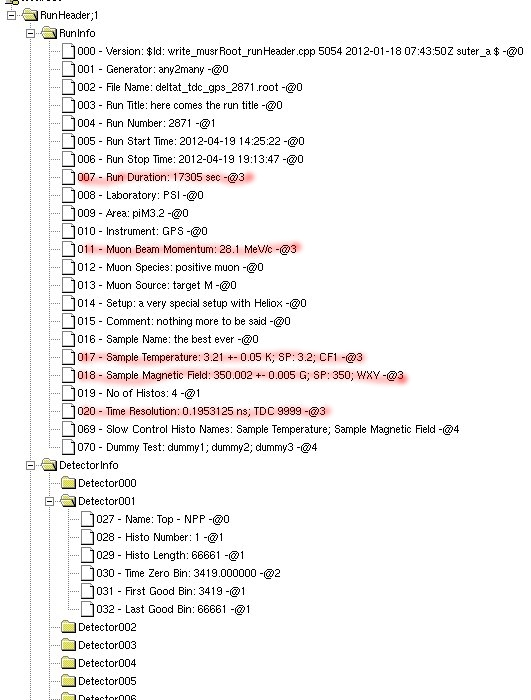
\includegraphics[width=0.7\textwidth]{MusrRootRunHeaderCartoon}
 \caption{\tmrh mock up. The red shaded entries are of type \texttt{TMusrRunPhysicalQuantity}.}\label{fig:MusrRootRunHeaderCartoon}
\end{figure}

\clearpage

\section{\tmrh Concept}\label{sec:tmrh_Concept}

The different \musr instruments need different information to be written into the data file (next to the most important ones: the histograms). The above defined properties are the \emph{minimal number of required} ones. There are different possible approaches to deal with it on the implementation level.

\begin{enumerate}
 \item A base class dealing with \emph{minimal required} standard is defined. Afterwards for each instrument a class is derived which is extending the base class to the needs of the instrument.
 \item The base class is defined in a more abstract way, and some external, text-based description is given which defines the details of the instrument.
\end{enumerate}

\noindent Even though the first approach is very clean, it would mean a lot of maintenance work. The 2nd approach is slightly more demanding for the handling class (\tmrh and helper classes), but having the advantage of easy maintainability and expandability. The idea is that all header information can be classified into 7 groups (see also tables in Sec.\ref{sec:RunInfo}, and Appendices \ref{sec:RunInfoRequired}--\ref{sec:BeamlineInfoRequired}): 

\begin{enumerate}
 \item strings, represented by \tstring
 \item integers, represented by \verb!Int_t!
 \item floating point numbers, represented by \verb!Double_t!
 \item physical quantities, represented by \tquant (see Appendix \ref{sec:TMusrRunPhysicalQuantity})
 \item collection of strings, represented by \tstringvec
 \item collection of integers, represented by \tintvec
 \item collection of floating point numbers, represented by \tdoublevec
\end{enumerate}

\noindent These properties can be collected by themselves in form of vectors. This way any needed information can be written into the \rootcern file. The class \tmrh is implementing this run header concept. In Sec. \ref{sec:UserInterface} code snippets will be discussed, showing how this is used on level of the \midas analyzer, \musrfit reader routine, \anytwomany conversion routines. Sec. \ref{sec:Validation} will discuss how to validate \musrroot files.

\subsection{User Interface for \musrroot Run Header}\label{sec:UserInterface}

There are two things needed to deal with the \musrroot run header, namely writing it and reading it. I will start with the writing as will be done in the \midas analyzer.

\subsubsection{Writing a \musrroot Run Header}\label{sec:UserInterfaceWritting}

An example program \verb!write_musrRoot_runHeader! which is writing a full run header is part of the \musrfit package. Here I will concentrate just on the most essential parts. First one needs an instance of \tmrh

\begin{shaded}
\begin{verbatim}  
TMusrRunHeader *header = new TMusrRunHeader();
TMusrRunPhysicalQuantity prop;
\end{verbatim}
\end{shaded}

\noindent \texttt{header} is the instance of \tmrh. \texttt{prop} is an instance of \tquant which will be needed further down in the description. In the next step some run header entries will be added

\begin{shaded}
\begin{verbatim}  
header->Set("RunInfo/File Name", "deltat_tdc_gps_2871.root");
header->Set("RunInfo/Run Title", "here comes the run title");
header->Set("RunInfo/Run Number", 2871);
\end{verbatim}
\end{shaded}

\noindent Adding information is done via the multiple overloaded \verb!Set(<pathName>,<value>)! method. Here \verb!<pathName>! is a string representing the ``path'' like representation in the \musrroot file structure, followed by the ``value'' to be set, \eg ``\texttt{File Name}''. \verb!<value>! can be any of the types listed at the beginning of Sec. \ref{sec:tmrh_Concept}. Here a few examples how to set \tquant.

\begin{shaded}
\begin{verbatim}  
prop.Set("Sample Temperature", 3.2, 3.21, 0.05, "K", "CF1");
header->Set("RunInfo/Sample Temperature", prop);

prop.Set("Time Resolution", 0.1953125, "ns", "TDC 9999");
header->Set("RunInfo/Time Resolution", prop);

prop.Set("CF3", MRH_UNDEFINED, 3.27, 0.09, "K", "strange temperature");
header->Set("SampleEnvironmentInfo/CF3", prop);
\end{verbatim}
\end{shaded}

\noindent Here \tquant objects are fed via the use of the overloaded set-method. For details see Appendix \ref{sec:TMusrRunPhysicalQuantity}.

\noindent To set some property within ``sub-sub-directories'' it would like this:

\begin{shaded}
\begin{verbatim}  
header->Set("DetectorInfo/Detector001/Time Zero Bin", 3419.0);
\end{verbatim}
\end{shaded}

\noindent To write the whole run header into a file would look something like this:

\begin{shaded}
\begin{verbatim}  
TFile *f = new TFile(fileName, "RECREATE", "write_musrRoot_runHeader");
if (f->IsZombie()) {
  delete f;
  return -1;
}

// create the needed TFolder object
TFolder *runHeader = new TFolder("RunHeader", "MusrRoot Run Header Info");

// create the "directory" structure
if (header->FillFolder(runHeader)) {
  runHeader->Write(); // write run header to file
}

f->Close();
\end{verbatim}
\end{shaded}


\subsubsection{Reading a \musrroot Run Header}\label{sec:UserInterfaceReading}

The following code snippet shows how the extract the full run header from the \musrroot file.

\begin{shaded}
\begin{verbatim}  
TFile *f = new TFile(fileName, "READ", "read_musrRoot_runHeader");
if (f->IsZombie()) {
  delete f;
  return -1;
}

TFolder *runHeader = 0;
f->GetObject("RunHeader", runHeader);
if (runHeader == 0) {
  cerr << endl << ">> **ERROR** Couldn't get top folder RunHeader";
  closeFile(f);
  return -1;
}

TMusrRunHeader *header = new TMusrRunHeader(fileName);

if (!header->ExtractAll(runHeader)) {
  cerr << endl << ">> **ERROR** couldn't extract all RunHeader information";
  closeFile(f);
  return -1;
}

f->Close();
delete f;
\end{verbatim}
\end{shaded}

\noindent The routine \texttt{ExtractAll(TFolder *runHeader)} decodes all the \tobjstring objects and fills internal data structures. This means when reading a \musrroot-file the above handling is always needed. After the \texttt{ExtractAll} call, parameters can be extracted via the getter routines available. For instance to read the ``Run Number'', the code would look like 

\begin{shaded}
\begin{verbatim}
Bool_t ok;
Int_t ival;  
header->Get("RunInfo/Run Number", ival, ok);
if (ok)
  cout << endl << "Run Number: " << ival;
else
  cout << endl << "**ERROR** Couldn't obtain the 'Run Number'.";
\end{verbatim}
\end{shaded}
 
\noindent Reading a \tquant object, \eg the ``Sample Temperature'' looks like this 

\begin{shaded}
\begin{verbatim}
TMusrRunPhysicalQuantity prop;

header->Get("RunInfo/Sample Temperature", prop, ok);
if (ok) {
  cout << endl << "Sample Temperature: " << prop.GetValue() << " +- ";
  cout << prop.GetError() << " " << prop.GetUnit().Data();
  cout << "; SP: " << prop.GetDemand() << "; " << prop.GetDescription().Data();
} else {
  cout << endl << "**ERROR** Couldn't obtain the 'Sample Temperature'.";
}
\end{verbatim}
\end{shaded}


\subsection{Validation of a \musrroot File}\label{sec:Validation}

In order to validate the information an additional mechanism is needed. There are various levels of validation: (i) is a given \rootcern-file a \musrroot-file? (ii) Contains the given \musrroot-file the \emph{minimum} of required entries needed? (iii) Is the given \musrroot-file for a given instrument compatible with the instrument specific definition? (iv) Do the given information make any sense?  

Point (iv) can only be judged by the person looking at the file and hence will not be discussed any further here. Points (i)-(iii) can be validated within ``XML Schema Validation'' framework \cite{xml-schema}. Why choosing XML Schema Validation? The advantage is that the \musrroot-file structure can be mapped onto an ASCII-file, containing all the validation information needed. Furthermore, the whole parser facilities are readily available for virtually all platforms. Who will need to deal with this validation stuff? This is valuable for persons which need to implement \musrroot-file writing on level of the instrument data acquisition or for guys writing data file converters, \ie just very few ones. 

\begin{figure}[h]
  \centering
  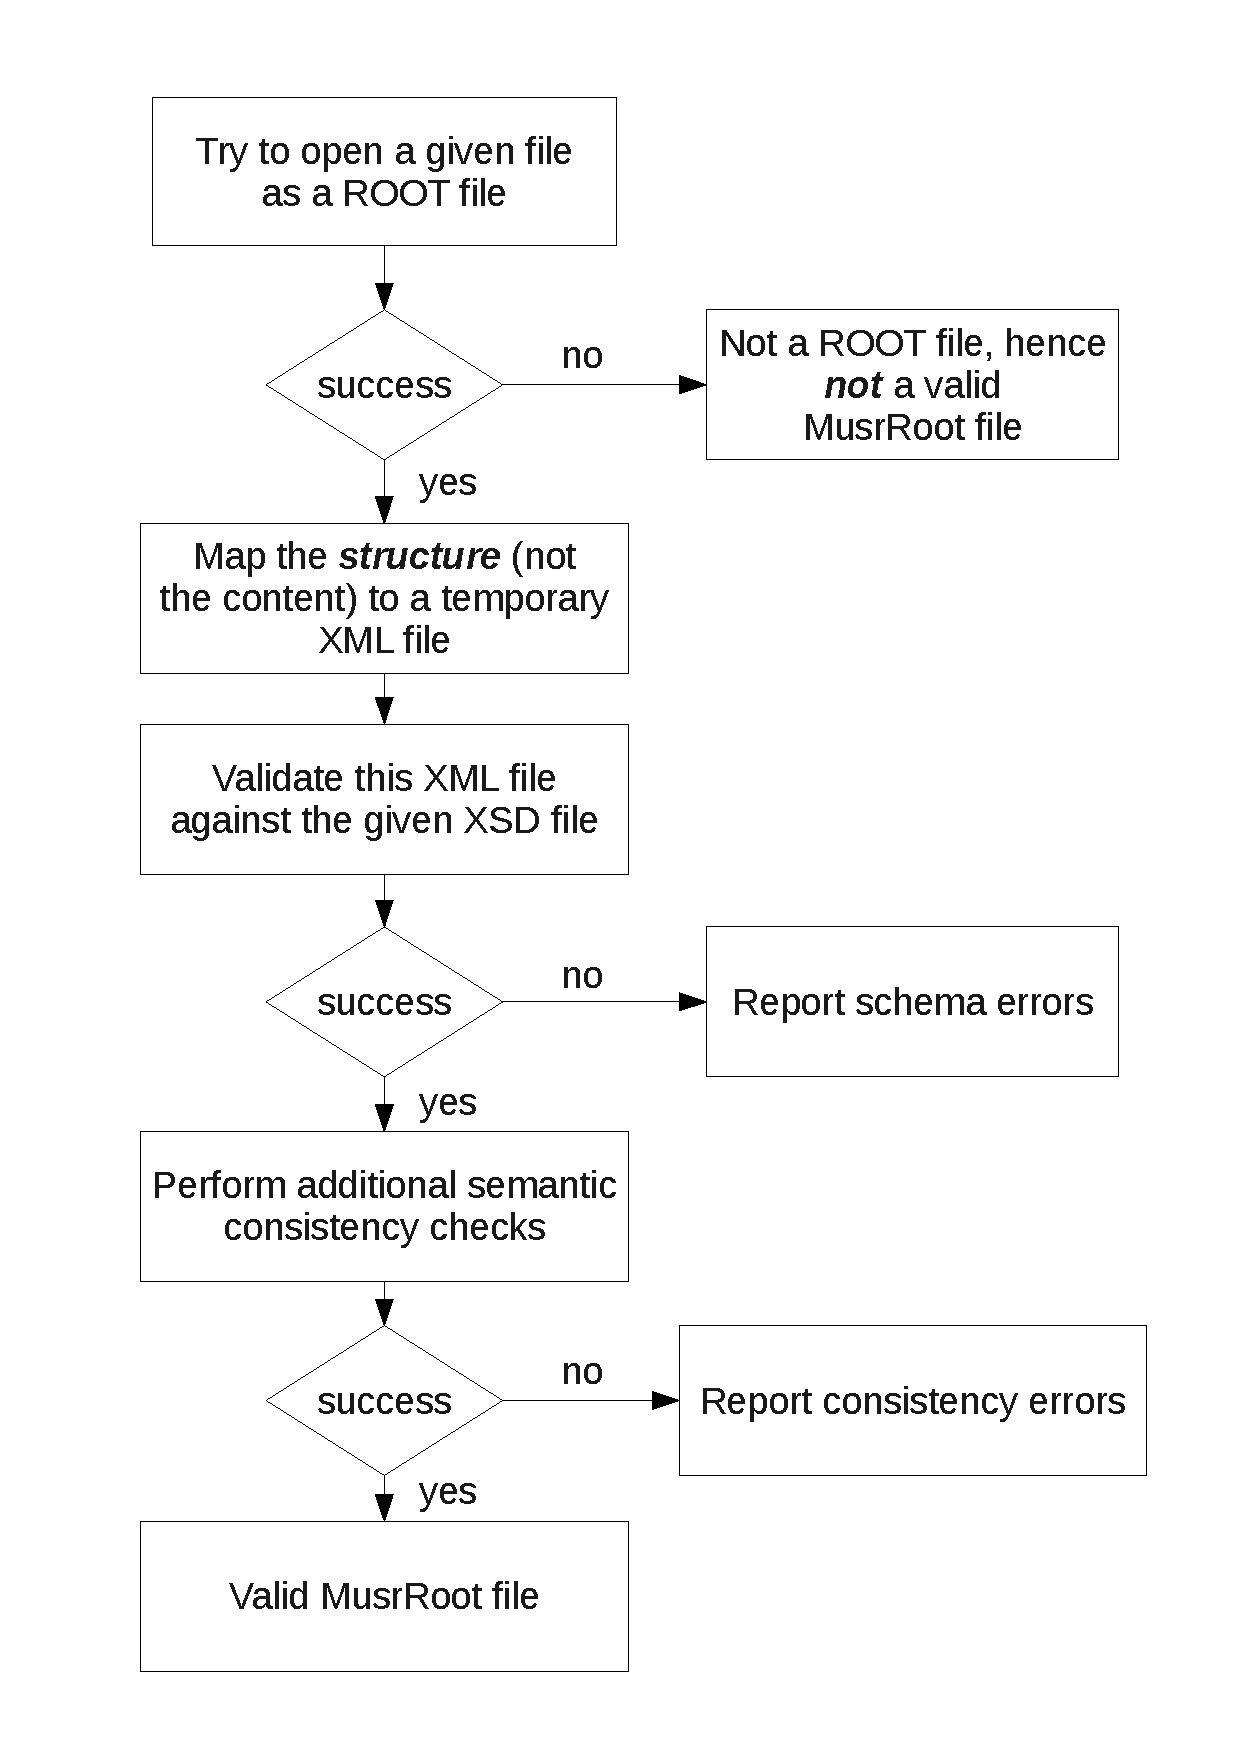
\includegraphics[width=0.7\textwidth]{MusrRootValidationScheme}
  \caption{\musrroot validation scheme}\label{fig:MusrRootValidation}
\end{figure}


In the following this validation scheme will be discussed as it is implemented (see also Fig.\ref{fig:MusrRootValidation}) in \texttt{musrRootValidation} :
\begin{enumerate}
   \item It is checked if the given file name is a TFile.
   \item The file structure is recursively parsed and mapped into an temporary XML file. XML is used since there are ample of parser and validation frameworks at hand. For details check any decent book about XML. Here the libxml2 is used, because also \rootcern is requiring it.
   \item In a next step the XML file (holding the structure of the supposed \musrroot file is validated against a XML schema. The minimum of required entries is described by \texttt{MusrRoot.xsd} which is part of musrfit but also available from the PSI/LMU web-page.
   \item If the schema validation is successful additional semantic checks (like is the number of decay histograms the same as the number of detector entries, etc.) will be preformed. 
\end{enumerate}

This validation scheme is useful for people which define instrument specific extensions of the base MusrRoot, as for instance the LEM instrument at PSI. It is also useful for people writing file converters in order to cross check if the generated file is valid. The generic \musrroot validation file is given in Appendix \ref{sec:ValidationFile}. 

There will be always 2 validation files, the generic one, which defines the \emph{minimum required} standard for \emph{all} \musr instruments. This will be called \texttt{MusrRoot.xsd}, and an instrument specific one, called \verb!MusrRoot<name>.xsd!, where \verb!<name>! is the instrument name. The generic \musrroot definition must be fully present in each instrument definition, \ie the instrument definition is always an \emph{extension} of the generic \musrroot-file definition.

All validation files need to be open to the community via web-page. The URL from where to download these files will be part of the run header itself (see Appendix \ref{sec:RunInfoRequired}).

\clearpage

\appendix

\section{RunInfo --- Required Items} \label{sec:RunInfoRequired}

\begin{small}
\begin{tabular}{l|l|l}
Name           & internal type & Comment \\ \hline\hline
Version        & \tstring      & SVN version of \tmrh \\
Generic Validator URL & \tstring & URL of the generic \musrroot validation xsd-file, \\
               &               & example given below $^1$. \\
Specific Validator URL & \tstring & URL of the instrument specific validation xsd-file$^2$ \\
Generator      & \tstring      & Program which wrote the \musrroot file, \\
               &               & \eg \verb!nemu_analyzer! \\
Proposal Number & \verb!Int_t! & This item is optional, but if present, it \\
               &               & can only occur once. \\
Main Proposer  & \tstring      & This item is optional, but if present, one \\
               &               & or more main proposers are possible. \\               
File Name      & \tstring      & File name of the \musrroot file, \\
               &               & \eg \verb!deltat_tdc_gps_4295.root! \\
Run Title      & \tstring      & \\
Run Number     & \verb!Int_t!  & \\
Run Start Time & \tstring      & ISO 8601 date time \\
Run Stop Time  & \tstring      & ISO 8601 date time \\
Run Duration   & \tquant       & run duration in sec \\
Laboratory     & \tstring      & \eg PSI \\
Instrument     & \tstring      & \eg GPS \\
Muon Beam Momentum & \tquant    & \eg $28.1\,\mathrm{MeV/c}$ \\
Muon Species   & \tstring      & positive, or negative muon \\
Muon Source    & \tstring      & \eg ``Target E -- Low Energy Muons'' or \\
               &               & ``Target E'' \ldots \\
Setup          & \tstring      & \\
Comment        & \tstring      & \\
Sample Name    & \tstring      & \\
Sample Temperature & \tquant    & \eg \verb!3.21 +- 0.05 K; SP: 3.2; CF1! \\
Sample Magnetic Field & \tquant & \eg \verb!350.002 +- 0.005 G; SP: 350; WXY! \\
No of Histos   & \verb!Int_t!  & \\
Time Resolution & \tquant       & \eg \verb!0.1953125 ns! \\
RedGreen Offsets & \tintvec & \eg \verb!0; 20! \\
\end{tabular}

\vspace{5mm}

\noindent $^1$ \eg \verb!http://lmu.web.psi.ch/facilities/software/MusrRoot/Validation/MusrRoot.xsd!

\noindent $^2$ \eg \verb!http://lmu.web.psi.ch/facilities/software/MusrRoot/Validation/MusrRootLEM.xsd!
\end{small}

\section{DetectorInfo --- Required Items} \label{sec:DetectorInfoRequired}

The \texttt{DetectorInfo} is organized in a sub-tree like

\begin{verbatim}
DetectorInfo ---|
                |-Detector001
                |-Detector002
                ...                
\end{verbatim}

\noindent For each histogram in the \verb!histos/DecayAnaModule! corresponds detector entry here. 

\noindent The numbering of the detectors has to correspond the its histogram, \eg \verb!hDecay023! $\leftrightarrow$ \verb!Detector023!, \ie potentially discontinuous to show \redgreen breaks.

\vspace{2mm}

\noindent \verb!Detector<XXX>! has the elements

\vspace{2mm}

\begin{tabular}{l|l|l}
Name           & internal type   & Comment \\ \hline\hline
Name           & \tstring        & detector name, \eg \texttt{Left - NPP} \\
Histo Number   & \verb!Int_t!    & histogram number$^1$ \\
Histo Length   & \verb!Int_t!    & length of the histogram \\
Time Zero Bin  & \verb!Double_t! & see comment $^2$ \\
First Good Bin & \verb!Int_t!    & \\
Last Good Bin  & \verb!Int_t!    & \\
\end{tabular}

\vspace{2mm}

\begin{small}
\noindent $^1$ This number corresponds to the histogram number in the \verb!histos/DecayAnaModule! sub-tree.

\noindent $^2$ The type is \verb!Double_t! since for the high-field spectrometer an \verb!Int_t! representation would be not good enough.
\end{small}

\section{SampleEnvironmentInfo --- Required Items} \label{sec:SampleEnvironmentInfoRequired}

Here only a single entry is required, namely 

\vspace{2mm}

\begin{tabular}{l|l|l}
Name           & internal type   & Comment \\ \hline\hline
Cryo           & \tstring        & name of the used cryostate, \eg \texttt{Konti-2} \\
\end{tabular}


\section{MagneticFieldEnvironmentInfo --- Required Items} \label{sec:MagneticFieldEnvironmentInfoRequired}

Here only a single entry is required, namely 

\vspace{2mm}

\begin{tabular}{l|l|l}
Name           & internal type   & Comment \\ \hline\hline
Magnet Name    & \tstring        & name of the used magnet$^1$, \eg \texttt{WEW} \\
\end{tabular}

\vspace{2mm}

\begin{small}
\noindent $^1$ In case of ZF measurements, there might be an entry as ``ZF''?
\end{small}

\section{BeamlineInfo --- Required Items} \label{sec:BeamlineInfoRequired}

Here only a single entry is required, namely 

\vspace{2mm}

\begin{tabular}{l|l|l}
Name           & internal type   & Comment \\ \hline\hline
Name           & \tstring        & name of the beamline, \eg \texttt{piM3.2} \\
\end{tabular}

\section{Exhaustive MusrRoot tree --- including everything \emph{required}}
Here it is assumed that there are \emph{hypothetical} \redgreen data with electric field on/off and light on/off, and hence 4 data sets per detector, and 8 detectors of the instrument: \texttt{left/forward, top/forward, right/forward, bottom/forward, left/backward, top/backward, right/backward, bottom/backward}. To show the whole tree structure, it will be splitted in the representation afterwards, but keep in mind: this will be all part of a single \musrroot file. I will add comments in the tree structure by the symbol \verb!#!. Lets start with the \musr data histograms:
\begin{small}
\begin{verbatim}
histos -|
        |- DecayAnaModule -|
                           |- hDecay001 # left/forward, electric field off, light off
                           |- hDecay002 # top/forward, electric field off, light off
                           |- hDecay003 # right/forward, electric field off, light off
                           |- hDecay004 # bottom/forward, electric field off, light off
                           ...
                           |- hDecay007 # right/backward, electric field off, light off
                           |- hDecay008 # bottom/backward, electric field off, light off
                           |- hDecay011 # left/forward, electric field on, light off
                           |- hDecay012 # top/forward, electric field on, light off
                           |- hDecay013 # right/forward, electric field on, light off
                           |- hDecay014 # bottom/forward, electric field on, light off
                           ...
                           |- hDecay017 # right/backward, electric field on, light off
                           |- hDecay018 # bottom/backward, electric field on, light off
                           |- hDecay021 # left/forward, electric field off, light on
                           |- hDecay022 # top/forward, electric field off, light on
                           |- hDecay023 # right/forward, electric field off, light on
                           |- hDecay024 # bottom/forward, electric field off, light on
                           ...
                           |- hDecay027 # right/backward, electric field off, light on
                           |- hDecay028 # bottom/backward, electric field off, light on
                           |- hDecay031 # left/forward, electric field on, light on
                           |- hDecay032 # top/forward, electric field on, light on
                           |- hDecay033 # right/forward, electric field on, light on
                           |- hDecay034 # bottom/forward, electric field on, light on
                           ...
                           |- hDecay037 # right/backward, electric field on, light on
                           |- hDecay038 # bottom/backward, electric field on, light on
                           ...
\end{verbatim}
\end{small}
\noindent Comments: as can be seen the histograms are continuous numbered until there is a \redgreen mode switch where the histogram number ``jumps'' (e.g. from \verb!008! to \verb!011!). In order to fill in the different \redgreen histograms an offset is added (here 10, 20, and 30).

Next there will be the slowcontrol histograms:
\begin{small}
\begin{verbatim}
histos -|
        |- SCAnaModule -|
                        |- hSampleTemperature
                        |- hMagneticField
                        |- hModeratorTemperature
                        ...
\end{verbatim}
\end{small}
\noindent Comments: Theses histograms show typical time histograms of temperature, magnetic field, etc. \emph{during} the run. The number of the histograms and their content will be quite different for each instrument.

Next the whole \texttt{RunHeader}. Here the information will be grouped in different folders collecting related information, like general run info, detector info, sample and magnetic field environment info, beamline info, etc.
\begin{small}
\begin{verbatim}
RunInfo:
  000 - Version: git-sha fec5017fc29 -@0
  001 - Generic Validator URL: http://lmu.web.psi.ch/facilities/software/MusrRoot/Validation/MusrRoot.xsd -@0
  002 - Specific Validator URL: http://lmu.web.psi.ch/facilities/software/MusrRoot/Validation/MusrRootLEM.xsd -@0
  003 - Generator: nemu_analyzer -@0
  004 - Proposal Number: 20190275 -@1
  005 - Main Proposer: John Doe -@0
  006 - File Name: lem12_his_0234.root -@0
  007 - Run Title: here comes the run title -@0
  008 - Run Number: 234 -@1
  009 - Run Start Time: 2012-04-19 14:25:22 -@0
  010 - Run Stop Time: 2012-04-19 19:13:47 -@0
  011 - Run Duration: 17305 sec -@3
  012 - Laboratory: PSI -@0
  013 - Instrument: LEM -@0
  014 - Muon Beam Momentum: 28.1 MeV/c -@3
  015 - Muon Species: positive muon -@0
  016 - Muon Source: target E -@0
  017 - Setup: a very special setup -@0
  018 - Comment: nothing more to be said -@0
  019 - Sample Name: the best ever -@0
  020 - Sample Temperature: 3.21 +- 0.05 K; SP: 3.2 -@3
  021 - Sample Magnetic Field: 350.002 +- 0.005 G; SP: 350 -@3
  022 - No of Histos: 8 -@1
  023 - Time Resolution: 0.1953125 ns;  TDC 9999 -@3
  024 - RedGreen Offsets: 0; 10; 20; 30
DetectorInfo:
  Detector001:
    025 - Name: Left/Forward - electric field off, light off -@0
    026 - Histo Number: 1 -@1
    027 - Histo Length: 66661 -@1
    028 - Time Zero Bin: 3419.000000 -@2
    029 - First Good Bin: 3419 -@1
    030 - Last Good Bin: 66661 -@1
  Detector002:
    031 - Name: Top/Forward - electric field off, light off -@0
    032 - Histo Number: 2 -@1
    033 - Histo Length: 66661 -@1
    034 - Time Zero Bin: 3419.000000 -@2
    035 - First Good Bin: 3419 -@1
    036 - Last Good Bin: 66661 -@1

  ...

  Detector038:
    213 - Name: Bottom/Backward - electric field on, light on -@0
    214 - Histo Number: 38 -@1
    215 - Histo Length: 66661 -@1
    216 - Time Zero Bin: 3419.000000 -@2
    217 - First Good Bin: 3419 -@1
    218 - Last Good Bin: 66661 -@1

SampleEnvironmentInfo:
  219 - Cryo: Konti-1 -@0
  220 - Insert: X123 -@0
  221 - Orientation: c-axis perp spin, perp field. spin perp field -@0
MagneticFieldEnvironmentInfo:
  222 - Magnet Name: WEW -@0
  223 - Current: 17.34 A -@3
BeamlineInfo:
  224 - Name: muE4 -@0
ScalerInfo:
  225 - Ip: 12332123 -@1
RunSummary:
  0000 - Wed Oct  5 01:30:37 2011 Run 2856 started.
  0001 - Wed Oct  5 02:02:51 2011 Run 2856 stopped.
  0002 - 
  0003 - LCO, T=170.02(K), wTF ~30(G)/5.18(A), Tr/Sa=15.02/8.50(kV), E=5.63(keV), LEDb off, BP off
  0004 - =========================================================================================
  0005 - 
  0006 - #BUC---- B e g i n of User Comment ------ Do not edit this line
  0007 - #EUC----   E n d   of User Comment ------ Do not edit this line
  0008 - 
  0009 - ======================   E v e n t  definition   =========================
  0010 -
  0011 - Events: 
  0012 - Event_0: (BC)-MCP1-(e+); Event_1:( BC)-TD-MCP2-(e+); Event_2: LEmuSR, (BC)-TD-e 
  ...
\end{verbatim}
\end{small}

\noindent Comment: the last sub-tree (\texttt{RunSummary}) is not following \tmrh rule \\ \verb!<number> - <label>: <value> -@<type>!. It is added in the instrument analyzer directly by other means than \tmrh \texttt{Set}-method. This is no problem! Since \texttt{RunSummary} is not part of the \emph{required} \musrroot-file. One is quite free in adding any \rootcern based information here.

\section{\tquant --- Possible Representations} \label{sec:TMusrRunPhysicalQuantity}

A physical property can be described as
  
\begin{leftbar}
\begin{verbatim}
<property name>: <value> +- <estimated error> <unit>; SP: <demand>; <description>
\end{verbatim}
\end{leftbar}

\noindent where \texttt{<property name>} is the name of the quantity, \eg \texttt{Sample Temperature},  \texttt{<value>} the value of the quantity, \texttt{<estimated error>} the error estimate, \eg the standard deviation, \texttt{<unit>} the unit, \eg K, \texttt{<demand>} a demand value, \eg the set point of the temperature. \texttt{<description>} is a possible additional comment for this quantity.

Note, not all of these quantities are always needed. The list of handled combination are given hereafter together with the \verb!C++! code snipped how to set it. It is assumed that \verb!TMusrRunPhysicalQuantity prop;! is somewhere defined.

\begin{leftbar}
\begin{verbatim}
<property name>: <value> <unit>[; <description>]
\end{verbatim}
\end{leftbar}

\begin{shaded}
\begin{verbatim}  
prop.Set("Muon Beam Momentum", 28.1, "MeV/c");
header->Set("RunInfo/Muon Beam Momentum", prop);

prop.Set("Time Resolution", 0.1953125, "ns", "TDC 9999");
header->Set("RunInfo/Time Resolution", prop);
\end{verbatim}
\end{shaded}

\noindent Result in the \texttt{RunHeader/RunInfo}:
\begin{verbatim}
011 - Muon Beam Momentum: 28.1 MeV/c -@3
013 - Time Resolution: 0.1953125 ns; TDC 9999 -@3 
\end{verbatim}

\noindent The number on front of the token (\eg \verb!011! in front of \verb!Muon Beam Momentum!) will depend on the position where the entry has been added. The last tokens, ``\verb!-@3!'', is the encoding of the type: here \tquant.

\noindent\hrulefill

\begin{leftbar}
\begin{verbatim}
<property name>: <val> +- <err> <unit>[; <description>]
\end{verbatim}
\end{leftbar}

\begin{shaded}
\begin{verbatim}  
prop.Set("CF3", MRH_UNDEFINED, 3.27, 0.09, "K", "strange temperature");
header->Set("SampleEnvironmentInfo/CF3", prop);
\end{verbatim}
\end{shaded}

\noindent Result in the \texttt{RunHeader/SampleEnvironmentInfo}:
\begin{verbatim}
033 - CF3: 3.27 +- 0.09 K; strange temperature -@3 
\end{verbatim}

\noindent\hrulefill

\begin{leftbar}
\begin{verbatim}
<property name>: <val> <unit>; SP: <demand>[; <description>]
\end{verbatim}
\end{leftbar}

\begin{shaded}
\begin{verbatim}  
prop.Set("CF4", 3.25, 3.28, "K");
header->Set("SampleEnvironmentInfo/CF4", prop);

prop.Set("CF5", 3.26, 3.29, "K", "another strange temperature");
header->Set("SampleEnvironmentInfo/CF5", prop);
\end{verbatim}
\end{shaded}

\noindent Result in the \texttt{RunHeader/SampleEnvironmentInfo}:
\begin{verbatim}
034 - CF4: 3.28 K; SP: 3.25 -@3
035 - CF5: 3.29 K; SP: 3.26; another strange temperature -@3
\end{verbatim}

\noindent\hrulefill

\begin{leftbar}
\begin{verbatim}
<property name>: <value> +- <estimated error> <unit>; SP: <demand>; <description>
\end{verbatim}
\end{leftbar}

\begin{shaded}
\begin{verbatim}  
prop.Set("Sample Magnetic Field", 350.0, 350.002, 0.005, "G", "WXY");
header->Set("RunInfo/Sample Magnetic Field", prop);
\end{verbatim}
\end{shaded}

\noindent Result in the \texttt{RunHeader/RunInfo}:
\begin{verbatim}
017 - Sample Magnetic Field: 350.002 +- 0.005 G; SP: 350.0; WXY -@3
\end{verbatim}

\section{Generic \musrroot Validation File}\label{sec:ValidationFile}

Below the ``generic'' \musrroot validation file is given.
\begin{shaded}
\begin{small}
\begin{verbatim}
<?xml version="1.0" encoding="UTF-8"?>
<xs:schema xmlns:xs="http://www.w3.org/2001/XMLSchema"> 
  <xs:annotation>
    <xs:documentation>
       This XSD document describes the muSR file structure for CERN/ROOT based files.
       In the following it will be called MusrRoot.
       It is currently the default standard for writting muSR data files at the 
       Paul Scherrer Institute.
          
       Author: Andreas Suter, andreas.suter@psi.ch          
    </xs:documentation>
  </xs:annotation>
    
  <xs:element name="MusrRoot" type="musrRoot"/>
  
  <xs:complexType name="musrRoot">
    <xs:sequence>
      <xs:element ref="histos"/>
      <xs:element name="RunHeader" type="runHeaderFolder"/>
      <xs:any processContents="skip" minOccurs="0" maxOccurs="unbounded"/> <!-- here can go any additional stuff you like -->
    </xs:sequence>  
  </xs:complexType>
    
  <xs:element name="histos">
    <xs:annotation>
       <xs:documentation>
         The histos folder is containing potentially various subfolders. 
         At least two subfolders, called DecayAnaModule, and SlowControlAnaModule,
         which holds the muSR decay histograms, must be present.
      </xs:documentation>
    </xs:annotation>
      
    <xs:complexType>
      <xs:sequence>
        <xs:element name="DecayAnaModule" type="decayHistoData"/>
        <xs:element name="SCAnaModule" type="slowControlHistoData"/>
        <xs:any processContents="skip" minOccurs="0" maxOccurs="unbounded"/> <!-- here can go any additional stuff you like -->
      </xs:sequence>
    </xs:complexType>
  </xs:element>
       
  <xs:complexType name="decayHistoData">
     <xs:sequence>
       <xs:element name="DecayHistoEntry" type="decayHistoEntry" minOccurs="1" maxOccurs="unbounded"/>
     </xs:sequence> 
  </xs:complexType>
    
  <xs:complexType name="decayHistoEntry">
     <xs:sequence>
       <xs:element name="HistoName" type="histoName"/>
       <xs:element name="HistoType" type="histoType"/>  
     </xs:sequence>      
  </xs:complexType>
    
  <xs:simpleType name="histoName">
      <xs:restriction base="xs:string">
        <xs:pattern value="hDecay([0-9]){3,}"/> <!-- this means hDecayXXX, where XXX are 3 digits -->
      </xs:restriction>
  </xs:simpleType>  
    
  <xs:simpleType name="histoType">
      <xs:restriction base="xs:string">
        <xs:pattern value="TH1F"></xs:pattern>
      </xs:restriction>
  </xs:simpleType>  
  
  <xs:complexType name="slowControlHistoData">
    <xs:sequence>
      <xs:element name="SlowControlHistoEntry" type="slowControlHistoEntry" minOccurs="1" maxOccurs="unbounded"/>
    </xs:sequence>
  </xs:complexType>

  <xs:complexType name="slowControlHistoEntry">
      <xs:sequence>
        <xs:element name="SlowControlName" type="xs:string"/>
        <xs:element name="SlowControlType" type="slowControlType"/>
      </xs:sequence>
  </xs:complexType>
       
  <xs:simpleType name="slowControlType">
    <xs:restriction base="xs:string">
      <xs:pattern value="TH1F"/>  
    </xs:restriction>  
  </xs:simpleType>  

  <xs:complexType name="runHeaderFolder">
    <xs:sequence>
      <xs:element name="RunInfo" type="runInfo"/>
      <xs:element name="DetectorInfo" type="detectorInfo"/>
      <xs:element name="SampleEnvironmentInfo" type="sampleEnvironmentInfo"/>
      <xs:element name="MagneticFieldEnvironmentInfo" type="magneticFieldEnvironmentInfo"/>
      <xs:element name="BeamlineInfo" type="beamlineInfo"/>
      <xs:any processContents="skip" minOccurs="0" maxOccurs="unbounded"/> <!-- here can go any additional stuff you like -->
    </xs:sequence>
  </xs:complexType>
  
  <xs:complexType name="runInfo">
    <xs:sequence>
      <xs:element name="Version" type="TString"/>
      <xs:element name="Generic_Validator_URL" type="TString"/>
      <xs:element name="Specific_Validator_URL" type="TString"/>
      <xs:element name="Generator" type="TString"/>
      <xs:element name="Proposal Number" type="Int_t" minOccurs="0" maxOccurs="1"/>
      <xs:element name="Main Proposer" type="TString" minOccurs="0" maxOccurs="unbounded"/>
      <xs:element name="File_Name" type="TString"/>
      <xs:element name="Run_Title" type="TString"/>
      <xs:element name="Run_Number" type="Int_t"/>
      <xs:element name="Run_Start_Time" type="TString"/>
      <xs:element name="Run_Stop_Time" type="TString"/>
      <xs:element name="Run_Duration" type="TMusrRunPhysicalQuantity"/>
      <xs:element name="Laboratory" type="TString"/>
      <xs:element name="Instrument" type="TString"/>
      <xs:element name="Muon_Beam_Momentum" type="TMusrRunPhysicalQuantity"/>
      <xs:element name="Muon_Species" type="TString"/>
      <xs:element name="Muon_Source" type="TString"/>
      <xs:element name="Setup" type="TString"/>
      <xs:element name="Comment" type="TString"/>
      <xs:element name="Sample_Name" type="TString"/>
      <xs:element name="Sample_Temperature" type="TMusrRunPhysicalQuantity"/>
      <xs:element name="Sample_Magnetic_Field" type="TMusrRunPhysicalQuantity"/>
      <xs:element name="No_of_Histos" type="Int_t"/>
      <xs:element name="Time_Resolution" type="TMusrRunPhysicalQuantity"/>
      <xs:element name="RedGreen_Offsets" type="TIntVector"/>
      <xs:any processContents="skip" minOccurs="0" maxOccurs="unbounded"/> <!-- here can go any additional stuff you like -->
    </xs:sequence>
  </xs:complexType>
 
  <xs:simpleType name="Int_t">
    <xs:restriction base="xs:string">
      <xs:pattern value="Int_t"/>
    </xs:restriction>
  </xs:simpleType>
 
  <xs:simpleType name="Double_t">
    <xs:restriction base="xs:string">
      <xs:pattern value="Double_t"/>
    </xs:restriction>
  </xs:simpleType>
  
  <xs:simpleType name="TString">
    <xs:restriction base="xs:string">
      <xs:pattern value="TString"/>
    </xs:restriction>
  </xs:simpleType> 
   
  <xs:simpleType name="TMusrRunPhysicalQuantity">
    <xs:restriction base="xs:string">
      <xs:pattern value="TMusrRunPhysicalQuantity"/>
    </xs:restriction>
  </xs:simpleType>
  
  <xs:simpleType name="TIntVector">
    <xs:restriction base="xs:string">
      <xs:pattern value="TIntVector"/>
    </xs:restriction>
  </xs:simpleType>
  
  <xs:complexType name="sampleEnvironmentInfo">
    <xs:sequence>
      <xs:element name="Cryo" type="TString"/>
      <xs:any processContents="skip" minOccurs="0" maxOccurs="unbounded"/> <!-- here can go any additional stuff you like -->          
    </xs:sequence>
  </xs:complexType>
  
  <xs:complexType name="magneticFieldEnvironmentInfo">
    <xs:sequence>
      <xs:element name="Magnet_Name" type="TString"/>
      <xs:any processContents="skip" minOccurs="0" maxOccurs="unbounded"/> <!-- here can go any additional stuff you like -->          
    </xs:sequence>
  </xs:complexType>

  <xs:complexType name="detectorInfo">
    <xs:sequence>
      <xs:element name="Detector" type="detector" maxOccurs="unbounded"/>
    </xs:sequence>
  </xs:complexType>
  
  <xs:complexType name="detector">
    <xs:sequence>
      <xs:element name="Name" type="TString"/>
      <xs:element name="Histo_Number" type="Int_t"/>
      <xs:element name="Histo_Length" type="Int_t"/>
      <xs:element name="Time_Zero_Bin" type="Double_t"/>
      <xs:element name="First_Good_Bin" type="Int_t"/>
      <xs:element name="Last_Good_Bin" type="Int_t"/>
      <xs:any processContents="skip" minOccurs="0" maxOccurs="unbounded"/> <!-- here can go any additional stuff you like -->      
    </xs:sequence>
  </xs:complexType>
  
  <xs:complexType name="beamlineInfo">
    <xs:sequence>
    	<xs:element name="Name" type="TString"/>
      <xs:any processContents="skip" minOccurs="0" maxOccurs="unbounded"/> <!-- here can go any additional stuff you like -->          
    </xs:sequence>
  </xs:complexType>
</xs:schema>
\end{verbatim}
\end{small}
\end{shaded}

\begin{thebibliography}{10}
\bibitem{Midas}
\texttt{http://midas.psi.ch}

\bibitem{ROOT}
R.~Brun and F.~Rademakers, Nucl. Instrum. Methods Phys. Res., Sect. A {\bf{389}}, 81--86 (1997).\\
\texttt{http://root.cern.ch/}

\bibitem{ROOT-Docu}
\texttt{http://root.cern.ch/drupal/content/users-guide}\\
\texttt{http://root.cern.ch/drupal/content/reference-guide}

\bibitem{NeXus}
\texttt{http://www.nexusformat.org} \\
\texttt{http://www.hdfgroup.org}

\bibitem{musrfit}
\texttt{http://lmu.web.psi.ch/facilities/software/musrfit/user/intranet.psi.ch/MUSR/WebHome.html}

\bibitem{xml-schema}
\texttt{http://www.w3.org/XML/Schema} \\
\texttt{http://www.w3schools.com/schema/}

\end{thebibliography}

\end{document}
